%set ukuran paper jadi a4 sama 12 pixel font
\documentclass[a4paper,12pt, left=3cm,right=2cm,bottom=2cm, bahasa]{article}
\usepackage{graphicx} % Required for inserting images
\usepackage[utf8]{inputenc}
\usepackage{times}
\usepackage{float}

\usepackage[autostyle]{csquotes}

%hyprlink desuwa
\usepackage{hyperref}
\hypersetup{
    colorlinks,
    citecolor=black,
    filecolor=black,
    linkcolor=black,
    urlcolor=black
}
%ganti jadi roman
\usepackage{times}

%set margin
 \usepackage{geometry}
 \geometry{margin=2cm}

%set bahasa indonesia
%\captionsbahasa
 \usepackage[american]{babel}


%biber dsw
 \usepackage[backend=biber,style=apa, sorting=none]{biblatex}
 %\usepackage[backend=bibtex, sorting=none]{biblatex}
 
 \addbibresource{ref.bib}



%set spacing 1.5
 \usepackage{setspace}
 \onehalfspacing{}
\usepackage{tocloft}

%bikin tabel berwarna
\usepackage[table,xcdraw]{xcolor}
\renewcommand{\cftpartleader}{\cftdotfill{\cftdotsep}}

%bikin judul utama centering
\usepackage{titlesec}
\titleformat{\section}[hang]{\normalfont\Large\bfseries}{\thesection}{1em}{\centering}
%idk harus pake date biar gak nongol di title
\date{}

%judul dokumen
\title{Proses Pembuatan Yogurt\\ Praktikum Bioteknologi Konvensional}

\begin{document}

%bikin judul jalan
\maketitle
%bikin page ini ga pake nomor
\thispagestyle{empty}
% logo
\begin{figure}[H]
    \centering
    
\includegraphics[width=0.3\linewidth]{images/sman1.png}
\end{figure}
%vertical space 2 cm

%nama penulis
\begin{center}
    Kelompok 2 : \\
    \begin{tabular}{ll}
         1.& Hasby Nauril Atoriq  \\
         2.& Aira Nabila Putri\\
         3.& Chantika Nabila \\
         4.& Fahriza Adrian Alhakim Kurnia \\
         5.& Putri Oktaviani \\
         6.& Khanza Putri Ramdani \\
         7.& Nazwa Nur Zoharoh \\
         8.& Muhammad Ryan Sopian \\
         9.& Raissa Almirah \\
         10.& Rima Marlina \\
         11.& Sidqi Adwakhairan Namina \\

    \end{tabular}\\
    \vspace{0.5cm}
    Kelas X-1\\
    \vspace{1cm}
    \textbf{PEMERINTAH DAERAH PROVINSI JAWA BARAT}\\
    \textbf{DINAS PENDIDIKAN}\\
    \textbf{SMA NEGERI 1}
    \textbf{CIWIDEY}\\
    \textbf{2024}
\end{center}
\onehalfspacing{}
%ganti nomor jadi romaj
\pagenumbering{Roman}
\setcounter{section}{1}
\pagebreak

    \section*{DAFTAR ISI}
    \addcontentsline{toc}{section}{\protect\numberline{}DAFTAR ISI}
% \end{center}
\renewcommand{\cftdot}{.}
\renewcommand{\contentsname}{}
\tableofcontents



\vspace{3cm}
\section*{DAFTAR PUSTAKA}
\addcontentsline{toc}{section}{\protect\numberline{}DAFTAR PUSTAKA}
\medskip
\printbibliography

\pagebreak
\pagenumbering{arabic}
\setcounter{page}{1}
\setcounter{section}{1}


\section*{BAB I \\PENDAHULUAN}
\addcontentsline{toc}{section}{\protect\numberline{}BAB I PENDAHULUAN}
\subsection{Latar Belakang}
%\addcontentsline{toc}{subsection}{\protect\numberline{}1.1 Latar Belakang}
Masa remaja, khususnya usia sekolah menengah atas (SMA), merupakan periode penting untuk pertumbuhan fisik, perkembangan kognitif, dan pematangan emosional. Asupan nutrisi yang berkualitas sangat diperlukan untuk mendukung aktivitas akademik dan kegiatan sehari-hari. Salah satu sumber nutrisi yang dianjurkan adalah yogurt, produk fermentasi susu yang kaya akan probiotik, protein, kalsium, dan vitamin. Probiotik dalam yogurt bermanfaat untuk kesehatan pencernaan dan imunitas, sedangkan kalsium dan protein mendukung pertumbuhan tulang dan otot\cite{Widi_et_al_2018}.

Namun, yogurt komersial yang beredar di pasaran seringkali mengandung tambahan gula, pengawet, atau perasa buatan yang kurang sehat jika dikonsumsi berlebihan. Di sisi lain, harga yogurt kemasan juga relatif mahal, sehingga kurang terjangkau bagi sebagian siswa. Oleh karena itu, pembuatan yogurt menggunakan susu murni dapat menjadi alternatif yang lebih sehat, ekonomis, dan transparan karena siswa dapat mengontrol bahan-bahan yang digunakan.

Praktikum ini juga memiliki nilai edukatif yang tinggi. Melalui proses fermentasi dengan bakteri Lactobacillus bulgaricus dan Streptococcus thermophilus, siswa dapat mempelajari konsep mikrobiologi, bioteknologi sederhana, serta perubahan kimia pada susu selama fermentasi. Kegiatan ini sejalan dengan kurikulum biologi SMA yang mencakup materi tentang mikroorganisme dan aplikasinya dalam kehidupan. Selain itu, praktikum ini melatih keterampilan praktis, kreativitas, dan pemahaman siswa mengenai pentingnya makanan sehat yang dapat diolah secara mandiri.
\subsection{Tujuan Praktikum}
Praktikum pembuatan yogurt dari susu murni ini bertujuan untuk:
\begin{itemize}
  \item Memahami prinsip dasar fermentasi susu menjadi yogurt melalui peran bakteri asam laktat.
  \item Menganalisis faktor-faktor yang memengaruhi keberhasilan proses fermentasi, seperti suhu, kebersihan alat, dan waktu inkubasi.
  \item Mengaplikasikan metode ilmiah dalam mengamati perubahan fisikokimia susu selama pembuatan yogurt (misalnya: perubahan pH, tekstur, dan rasa).
  \item Menghasilkan yogurt sehat tanpa bahan tambahan sintetis yang dapat dikonsumsi sebagai alternatif camilan bergizi bagi siswa.
\end{itemize}
\subsection{Manfaat Praktikum}
Praktikum ini memberikan manfaat teoritis dan praktis, antara lain:
\begin{enumerate}
  \item Manfaat teoritis
    \begin{itemize}
    \item Siswa memahami konsep fermentasi, peran mikroorganisme dalam bioteknologi pangan, serta nutrisi dalam susu dan yogurt.
    \item Meningkatkan pengetahuan tentang pentingnya probiotik bagi kesehatan pencernaan dan imunitas tubuh.
    \end{itemize}
  \item Manfaat praktis
    \begin{itemize}
   \item Siswa terampil membuat yogurt sederhana menggunakan bahan alami, sehingga dapat diaplikasikan di rumah sebagai camilan sehat.
   \item Mengembangkan keterampilan laboratorium, seperti sterilisasi alat, pengukuran pH, dan pengamatan ilmiah.
   \item Mendorong kreativitas dalam modifikasi rasa yogurt menggunakan buah atau madu alami.
   \item Menanamkan kesadaran tentang keamanan pangan dan gaya hidup sehat melalui konsumsi produk olahan mandiri.
    \end{itemize}
\end{enumerate}
\pagebreak
%bab 2
\setcounter{subsection}{0}
\setcounter{section}{2}
\section*{BAB II \\ Bahan dan Metode Praktikum}
\addcontentsline{toc}{section}{\protect\numberline{}BAB II Bahan dan Metode Praktikum}
\subsection{Definisi Yogurt}
Yoghurt adalah susu yang dibuat melalui proses fermentasi bakteri dan dapat di buat dari susu apa saja (susu sapi murni, susu sapi UHT yang biasa di jual di supermarket, dan susu lainnya). Yoghurt mengandung dua jenis probiotik, yaitu \textit{Lactobacillus bulgaricus} dan streptococcus thermophillus. Tak hanya enak, ternyata yoghurt juga memiliki manfaat lain yang tidak diketahui. Kandungan gizi yang terdapat pada yoghurt sangat banyak.
Yoghurt merupakan minuman kesehatanyang terbuat dari olahan susu yang difermentasikan. yoghurt tidak hanya identik dengan rasa asamnya saja, tetapi dapat dipadukan dengan rasa manis dan dapat juga di tambahkan dengan sari-sari buah.
\subsection{Manfaat Yoghurt bagi kesehatan}
\begin{enumerate}
\item Menyehatkan pencernaan
\item Mengurangi risiko terjadinya infeksi pada vagina
\item Meremajakan wajah
\item Pembersih yang ramah lingkungan
\item Menurunkan risiko darah tinggi
\item Menjaga jantung tetap sehat
\item Mencegah osteoporosis
\item Mengendalikan berat badan
\item Melancarkan buang air besar
\item Mampu meredakan stress
\item Dan lainnya
\end{enumerate}
\pagebreak
%bab 3
% weird shit, harus pake 0
\setcounter{subsection}{0}
\setcounter{section}{3}
\section*{BAB III \\ Bahan dan Metode Praktikum}
\addcontentsline{toc}{section}{\protect\numberline{}BAB III Bahan dan Metode Praktikum}
\subsection{Tempat dan Waktu Praktikum}
\begin{tabular}{ll}
    Tempat Praktikum & : Rumah Sidqi adwakhairan namina \\
    Tanggal Praktikum & : Senin 3 Februari 2025 \\
  \end{tabular}\\

Jadwal Praktikum: 
\begin{center}
  \begin{table}[H]
  \begin{tabular}{|c|c|c|}
    \hline
    No & Tanggal & Kegiatan \\
    \hline
    1 & Minggu 2 Februari & Pembelian Bahan dan Alat \\
    2 & Senin 3 Februari & pelaksanaan Praktikum \\ 
    3 & Kamis 6 Februari & Penulisan Laporan \\
    \hline
  \end{tabular}\\
\end{table}
\end{center}


\subsection{Bahan dan Alat}
Bahan-bahan dan alat yang digunakan adalah sebagai berikut:
\begin{enumerate}
  \item Susu murni 250 ML
  \item Yogurt Biokul 1 Pcs
  \item Toples penyimpanan
  \item Kulkas 2 Pintu
  \item Kain Lap penutup
  \item Kompor Gas
  \item Panci
  \item spatula
\end{enumerate}
\pagebreak
\subsection{Langkah-Langkah Praktikum}
Langkah-langkah dalam praktik membuat yogurt sebagai Berikut:
\begin{enumerate}
\item Persiapkan bahan 
  \begin{figure}[H]
  \begin{center}
    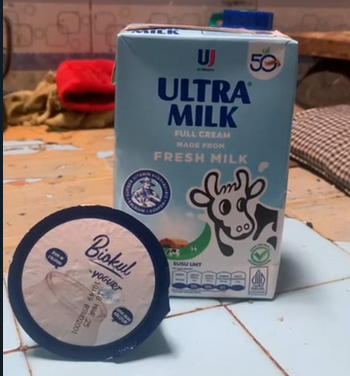
\includegraphics[width=0.5\textwidth]{images/gambar5.png}
  \end{center}
\end{figure}
\item  Masukan    Susu    Murni   ke      dalam     panci                                                     
  \begin{figure}[H]
  \begin{center}
    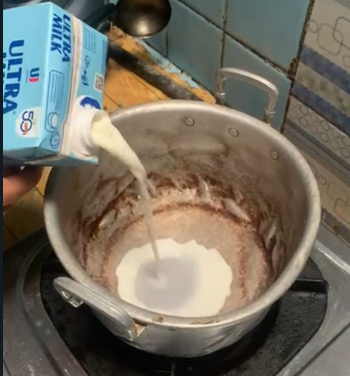
\includegraphics[width=0.5\textwidth]{images/gambar1.png}
  \end{center}
\end{figure}
\item  Panaskan   susu    murni   hingga  80        derajat  celsius                                          
  \begin{figure}[H]
  \begin{center}
    
\includegraphics[width=0.5\textwidth]{images/gambar2.png}
  \end{center}
\end{figure}
\item  Diamkan    susu    murni   hingga  40        derajat  celsius                                          
\item  Masukan    yogurt  ke      dalam   susu                                                                
  \begin{figure}[H]
  \begin{center}
    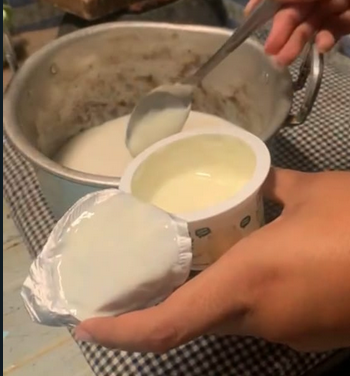
\includegraphics[width=0.5\textwidth]{images/gambar3.png}
  \end{center}
\end{figure}
\item  Masukan    susu    yang    telah   dicampur  yogurt   ke           dalam    wadah                      
\item  Selimuti   wadah   dengan  kain    lap       agar     tidak        terkena  cahaya  dan  harus  kedap  udara
  \begin{figure}[H]
  \begin{center}
    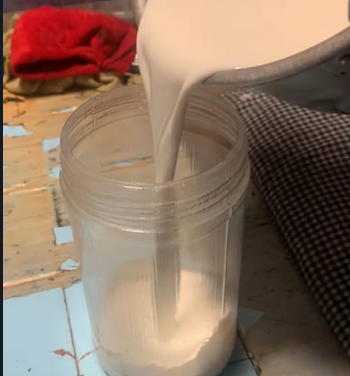
\includegraphics[width=0.5\textwidth]{images/gambar4.png}
  \end{center}
\end{figure}
\item  Simpan     bahan   selama  24      jam                                                                 
\item  Keluarkan  bahan   dari    wadah   dan       siap     dihidangkan                                      
  \begin{figure}[H]
  \begin{center}
    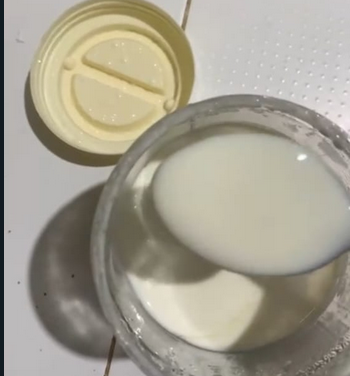
\includegraphics[width=0.5\textwidth]{images/gambar7.png}
  \end{center}
\end{figure}

\end{enumerate}

\setcounter{subsection}{0}
\setcounter{section}{4}
\section*{BAB IV \\ Hasil dan Pembahasan}
\addcontentsline{toc}{section}{\protect\numberline{}BAB IV Hasil dan Pembahasan}
\subsection{Hasil Praktikum}
Hasil dari praktikum ini adalah menghasilkan susu yang telah di fermentasi yang menjadikan susu tersebut menjadi yogurt, 
Setelah proses inkubasi selama 24 jam, susu murni yang telah dicampur dengan yogurt Biokul mengalami perubahan tekstur dan rasa. Susu yang awalnya cair berubah menjadi kental dan memiliki rasa asam yang khas. Perubahan ini menunjukkan bahwa proses fermentasi telah berhasil. Yogurt yang dihasilkan memiliki tekstur yang creamy dan rasa asam yang segar.
\subsection{pembahasan}
Praktikum ini berhasil membuat yogurt dari susu murni dengan menggunakan starter yogurt Biokul. Keberhasilan ini tidak lepas dari peran bakteri asam laktat (Lactobacillus bulgaricus dan Streptococcus thermophilus) yang terkandung dalam starter. Bakteri-bakteri ini memfermentasi laktosa (gula susu) menjadi asam laktat. Asam laktat inilah yang menyebabkan susu menjadi asam dan mengkoagulasi protein susu, sehingga menghasilkan tekstur kental pada yogurt.

Suhu inkubasi yang sangat penting untuk pertumbuhan bakteri. Suhu yang terlalu rendah dapat menghambat pertumbuhan bakteri, sedangkan suhu yang terlalu tinggi dapat mematikan bakteri. Pada praktikum ini, inkubasi dilakukan pada suhu ruang selama 24 jam. Suhu ruang di Indonesia umumnya berkisar antara 25-30°C, yang cukup ideal untuk fermentasi yogurt.

Selain suhu, kebersihan alat dan bahan juga berpengaruh pada keberhasilan fermentasi. Alat dan bahan yang tidak bersih dapat terkontaminasi oleh bakteri lain yang tidak diinginkan, yang dapat mengganggu pertumbuhan bakteri asam laktat dan menghasilkan yogurt yang tidak berkualitas. Oleh karena itu, sebelum digunakan, semua alat dan bahan yang digunakan dalam praktikum ini telah dicuci bersih dan disterilkan.

Waktu inkubasi 24 jam juga merupakan waktu yang untuk fermentasi yogurt. Waktu yang terlalu singkat dapat menghasilkan yogurt yang kurang asam dan kurang kental, sedangkan waktu yang terlalu lama dapat menghasilkan yogurt yang terlalu asam.
\pagebreak
\setcounter{subsection}{0}
\setcounter{section}{5}
\section*{BAB V \\ Penutup}
\addcontentsline{toc}{section}{\protect\numberline{}BAB V Penutup}
\subsection{Kesimpulan}
Berdasarkan hasil praktikum dan pembahasan yang telah diuraikan, dapat ditarik kesimpulan sebagai berikut:
\begin{enumerate}
  \item Praktikum pembuatan yogurt dari susu murni dengan menggunakan starter yogurt Biokul telah berhasil dilakukan.  Proses fermentasi oleh bakteri asam laktat (Lactobacillus bulgaricus dan Streptococcus thermophilus) dalam starter yogurt Biokul telah mengubah laktosa menjadi asam laktat, yang menyebabkan susu mengental dan menghasilkan rasa asam khas yogurt 
  \item yogurt yang dihasilkan memiliki karakteristik tekstur kental, rasa asam yang segar, dan aroma yang khas, sesuai dengan ciri-ciri yogurt pada umumnya.
  \item Faktor-faktor seperti suhu inkubasi, kebersihan alat dan bahan, serta waktu inkubasi memiliki peran penting dalam keberhasilan proses fermentasi dan kualitas yogurt yang dihasilkan.  Pada praktikum ini, suhu ruang (sekitar 25-30°C) dan waktu inkubasi 24 jam terbukti cukup optimal untuk menghasilkan yogurt yang baik.
\end{enumerate}
\subsection{Saran}
Berdasarkan pengalaman selama praktikum dan analisis hasil, beberapa saran dapat diajukan untuk perbaikan dan pengembangan lebih lanjut:
\begin{enumerate}
  \item Variasi Kondisi Fermentasi:  Untuk penelitian lebih lanjut, disarankan untuk melakukan percobaan dengan variasi suhu inkubasi dan waktu inkubasi yang berbeda. Hal ini bertujuan untuk mengetahui pengaruh kedua faktor tersebut secara lebih detail terhadap kualitas yogurt yang dihasilkan, seperti tingkat keasaman, tekstur, dan aroma.  Misalnya, dapat dicoba inkubasi pada suhu yang sedikit lebih rendah atau lebih tinggi, atau dengan waktu inkubasi yang lebih singkat atau lebih lama. 
  \item Penggunaan Starter yang Berbeda:  Selain yogurt Biokul, dapat juga dicobakan starter yogurt dari merek lain atau kultur murni bakteri Lactobacillus bulgaricus dan Streptococcus thermophilus secara terpisah.  Perbandingan hasil yogurt yang dihasilkan dengan starter yang berbeda dapat memberikan informasi mengenai pengaruh jenis starter terhadap kualitas yogurt. 
  \item Pengujian Kualitas Yogurt:  Untuk analisis yang lebih komprehensif, disarankan untuk melakukan pengujian kualitas yogurt secara lebih lanjut.  Pengujian ini dapat meliputi pengukuran pH untuk mengetahui tingkat keasaman, pengujian viskositas untuk mengetahui tingkat kekentalan, dan pengujian jumlah bakteri asam laktat untuk mengetahui viabilitas dan konsentrasi bakteri baik dalam yogurt.
  \item Penambahan Bahan Alami:  Untuk meningkatkan nilai gizi dan variasi rasa yogurt, dapat dicobakan penambahan bahan-bahan alami seperti buah-buahan segar, madu, atau ekstrak bahan alami lainnya setelah proses fermentasi selesai.  Penambahan ini perlu dilakukan dengan hati-hati agar tidak mengganggu kualitas yogurt.
  \item Sterilisasi yang Lebih Optimal:  Meskipun pada praktikum ini kebersihan alat dan bahan sudah diperhatikan, sterilisasi yang lebih optimal, seperti penggunaan autoklaf atau metode sterilisasi lainnya, dapat dipertimbangkan untuk memastikan tidak ada kontaminasi bakteri lain yang tidak diinginkan.
  \item Dokumentasi yang Lebih Baik:  Untuk praktikum selanjutnya, disarankan untuk melakukan dokumentasi yang lebih baik, termasuk pengambilan foto atau video pada setiap tahapan proses pembuatan yogurt. Dokumentasi ini akan sangat membantu dalam analisis hasil dan penyusunan laporan.
\end{enumerate}
\end{document}
